\section{Informazioni generali}
\subsection{Descrizione}
Il W3C\glo Data Model comprende diversi standard e tecnologie utilizzate per rappresentare e gestire dati strutturati nel contesto del Web semantico. Uno dei componenti principali di questo modello è il Resource Description Framework (RDF), che definisce una specifica per rappresentare le informazioni sul Web in un formato standardizzato. RDF si basa su un modello di dati basato su grafi, in cui le risorse web vengono descritte utilizzando triple, composte da un soggetto, un predicato e un oggetto. Queste triple RDF consentono di creare connessioni tra le risorse web e stabilire relazioni tra di esse. 
Un altro elemento chiave del W3C Data Model è il Web Ontology Language (OWL), che è un linguaggio di modellazione ontologica standardizzato. OWL offre un modo formale per descrivere i concetti, le proprietà e le relazioni tra gli oggetti all'interno di un dominio specifico. Utilizzando OWL, è possibile creare ontologie, che sono modelli concettuali che rappresentano la conoscenza di un dominio specifico. Le ontologie consentono di definire in modo preciso e strutturato i concetti e le relazioni all'interno del dominio, facilitando l'interoperabilità e l'integrazione dei dati.
Per l'interrogazione dei dati RDF, il W3C Data Model utilizza SPARQL, un linguaggio di interrogazione standardizzato. SPARQL consente di formulare query complesse per estrarre informazioni specifiche da un grafo RDF. Con SPARQL, è possibile eseguire query basate su pattern, che consentono di trovare risorse che soddisfano determinate condizioni. Inoltre, SPARQL supporta il ragionamento inferenziale, che consente di dedurre nuove informazioni dai dati RDF esistenti, e filtri per restringere ulteriormente i risultati delle query.\\
Uno degli obiettivi principali del W3C Data Model è consentire l'interoperabilità semantica tra diverse fonti di dati e applicazioni. Utilizzando gli standard del W3C, è possibile definire ontologie comuni, collegare dati provenienti da fonti diverse e consentire una comprensione e una condivisione dei dati coerenti.
In sintesi, il W3C Data Model offre un insieme di standard e tecnologie, tra cui RDF, OWL e SPARQL, per rappresentare, descrivere e interrogare dati strutturati nel contesto del Web semantico. Questi componenti consentono di creare connessioni tra le risorse web, definire ontologie per modellare la conoscenza di un dominio e interrogare i dati RDF per estrarre informazioni specifiche. L'uso di questo modello favorisce l'interoperabilità, la scoperta di conoscenza e l'integrazione dei dati in diversi settori e applicazioni.\\

Il W3C Data Model è implementato utilizzando un triplestore, un tipo di database che memorizza e gestisce triple RDF. Questo triplestore fornisce funzionalità per l'inserimento, l'aggiornamento, la ricerca e l'interrogazione dei dati RDF. I dati vengono organizzati in grafi RDF, che sono composti da triple RDF connesse tra loro. Ogni tripla rappresenta una relazione tra una risorsa (soggetto), una proprietà (predicato) e un valore o un'altra risorsa (oggetto).
Il W3C Data Model è basato su standard sviluppati e pubblicati dal World Wide Web Consortium (W3C), un'organizzazione che definisce standard aperti per il Web. Le specifiche RDF, OWL e SPARQL sono state pubblicate come raccomandazioni ufficiali dal W3C, garantendo l'interoperabilità e la compatibilità tra le diverse implementazioni.
Il modello di dati del W3C viene ampiamente utilizzato nel contesto del Web semantico e del Web delle cose. Grazie alla sua struttura flessibile e semantica, consente l'integrazione di dati provenienti da diverse fonti e domini, facilitando la condivisione e la scoperta di informazioni significative.
Oltre ai componenti principali, il W3C Data Model include anche altre specifiche correlate come RDFS (RDF Schema), che fornisce una struttura per la creazione di ontologie più semplici, e JSON-LD\glo, che permette l'incorporamento dei dati RDF all'interno di documenti JSON.
In conclusione, il W3C Data Model rappresenta un fondamento cruciale per l'implementazione di soluzioni basate sul Web semantico. Attraverso la sua struttura di triple RDF, la capacità di ragionamento inferenziale e l'interoperabilità garantita dalle specifiche del W3C, il modello di dati del W3C consente la rappresentazione, l'integrazione e l'interrogazione dei dati strutturati nel contesto del Web.\\

Nel contesto del W3C Data Model, i namespaces vengono utilizzati per identificare univocamente gli elementi all'interno di un grafo RDF. Questo evita collisioni di nomi e consente l'interoperabilità tra diverse ontologie e dataset RDF. Le ontologie, modelli di conoscenza formali, descrivono i concetti, le proprietà e le relazioni all'interno di un dominio specifico. Sono spesso create utilizzando il linguaggio OWL e consentono di definire gerarchie di classi, proprietà e restrizioni, facilitando l'interrogazione e l'inferenza sui dati RDF.
Il W3C Data Model ha avuto un impatto significativo sull'iniziativa Linking Open Data, che mira a creare un Web di dati interconnessi e aperti. Le risorse e i dataset vengono collegati utilizzando triple RDF, consentendo la scoperta e l'integrazione di dati provenienti da fonti diverse.\\
Il W3C Data Model è soggetto a continua evoluzione e miglioramento: le specifiche RDF, OWL e SPARQL vengono estese e migliorate per soddisfare le esigenze emergenti nel campo del Web semantico e dei dati collegati.
Il W3C Data Model trova applicazione in vari settori, come la pubblicazione di dati aperti, l'integrazione di dati eterogenei, la creazione di motori di ricerca semantici, la realizzazione di sistemi di raccomandazione personalizzati, l'analisi dei dati e la scoperta di conoscenze nascoste.\\

Il W3C Data Model è strettamente collegato al concetto di Linked Data, che si riferisce alla pratica di collegare dati strutturati all'interno del Web utilizzando gli standard del W3C, come RDF, per consentire la scoperta e l'interconnessione dei dati. Il W3C Data Model fornisce le fondamenta concettuali e tecniche per l'implementazione di Linked Data.
Il W3C Data Model consente la validazione dei dati RDF attraverso l'uso di schemi di validazione, come RDF Schema (RDFS) o OWL. Questi schemi definiscono le strutture e le restrizioni dei dati, consentendo di verificare la correttezza dei dati rispetto al modello specificato.\\
Esistono diversi linguaggi di serializzazione che possono essere utilizzati per rappresentare i dati RDF in formati leggibili da macchine e da esseri umani, come RDF/XML, Turtle, N-Triples e JSON-LD.
Il W3C Data Model è progettato per essere scalabile e adattarsi a un'ampia gamma di scenari e domini applicativi. La struttura flessibile dei grafi RDF, l'utilizzo di triple e la possibilità di espandere l'ontologia consentono di gestire grandi quantità di dati e di adattarsi alle esigenze in continua evoluzione.\\

Il W3C Data Model si integra con altri importanti standard del W3C, come HTML (Hypertext Markup Language), XML (eXtensible Markup Language) e XML Schema. Questa integrazione permette di incorporare i dati strutturati nel contesto delle pagine web, facilitando l'interazione tra dati e contenuti web.
Nel W3C Data Model, esistono ontologie comuni che vengono utilizzate in diversi ambiti e settori. Alcuni esempi includono FOAF\glo (Friend of a Friend) per la rappresentazione di informazioni sociali, Dublin Core\glo per la descrizione di risorse digitali e schema.org\glo per l'annotazione semantica dei contenuti web.
Il W3C Data Model consente di esprimere conoscenza strutturata nel contesto del Web. Attraverso l'utilizzo di ontologie, triple RDF e ragionamento inferenziale, è possibile rappresentare concetti complessi, relazioni e restrizioni, fornendo un'infrastruttura per la gestione di dati semanticamente ricchi.
Il W3C Data Model permette di collegare tra loro diverse risorse nel Web. Utilizzando le triple RDF, è possibile stabilire collegamenti tra risorse simili, creare aggregazioni di dati provenienti da fonti diverse e facilitare la scoperta di informazioni correlate.
Nel contesto del W3C Data Model, i vocabolari controllati sono utilizzati per definire le proprietà e i valori utilizzati nelle triple RDF. I vocabolari controllati forniscono un modo standardizzato e condiviso per rappresentare concetti e terminologia specifici di un dominio, garantendo l'interoperabilità e la comprensione condivisa dei dati.
Il W3C Data Model offre un approccio per l'integrazione di dati provenienti da fonti eterogenee. Attraverso l'uso di triple RDF e ontologie condivise, è possibile creare collegamenti tra dati provenienti da sorgenti diverse e combinare informazioni per ottenere una visione più completa dei dati.
Il W3C Data Model svolge un ruolo importante nella pubblicazione di dati aperti nel Web. Utilizzando gli standard RDF, è possibile pubblicare dati in un formato standardizzato, consentendo la condivisione, la riutilizzazione e l'integrazione dei dati da parte di terze parti.
Il W3C continua a sviluppare e migliorare il Data Model per affrontare le sfide emergenti e tenere il passo con le evoluzioni tecnologiche. Ciò include l'espansione dei vocabolari controllati, il miglioramento delle prestazioni delle query SPARQL e l'integrazione con nuovi domini e settori.\\

Il W3C Data Model permette l'annotazione semantica dei contenuti web, consentendo di aggiungere significato e contesto alle informazioni presenti sul Web. Attraverso l'uso delle triple RDF e delle ontologie, è possibile associare metadati semantici ai contenuti web, facilitando la ricerca, la comprensione e l'interoperabilità dei dati.\\
Il W3C Data Model offre strumenti e tecnologie per esplorare e navigare all'interno dei dati RDF. Attraverso le query SPARQL è possibile formulare interrogazioni complesse per estrarre informazioni specifiche dai grafi RDF e ottenere risposte basate sulle relazioni semantiche tra i dati.\\
Il W3C Data Model affronta anche questioni di privacy e sicurezza nell'ambito della gestione dei dati. Attraverso l'utilizzo di politiche di accesso controllato, crittografia e tecnologie di autenticazione, è possibile garantire che i dati vengano trattati in modo sicuro e rispettoso della privacy degli utenti.\\
Esistono una varietà di strumenti e librerie disponibili per lavorare con il W3C Data Model. Questi strumenti offrono funzionalità per la creazione, la gestione, l'interrogazione e la visualizzazione di dati RDF, semplificando lo sviluppo di applicazioni basate sul Web semantico. \\

Il W3C Data Model consente l'esportazione e l'importazione dei dati RDF in diversi formati. È possibile convertire i dati da un formato di serializzazione RDF a un altro per facilitare lo scambio e l'integrazione dei dati tra diverse applicazioni e sistemi.\\
Il W3C Data Model promuove l'adozione di best practice per la modellazione dei dati RDF. Ciò include l'uso di URI (Uniform Resource Identifier) univoci per identificare le risorse, l'utilizzo di vocabolari controllati consolidati e la creazione di ontologie ben strutturate per garantire l'interoperabilità e la reusabilità dei dati.\\
Il W3C Data Model è sostenuto da un processo di standardizzazione e governance guidato dal W3C. Questo assicura che gli standard correlati al modello di dati siano sviluppati in modo aperto, trasparente e collaborativo, coinvolgendo diverse parti interessate per garantire l'adozione e l'evoluzione continua degli standard.\\

Nonostante i numerosi vantaggi, il W3C Data Model presenta alcune sfide e limitazioni. Queste possono includere la complessità nella creazione di ontologie ben strutturate, la gestione di grandi quantità di dati RDF e la necessità di competenze specializzate per lavorare con i concetti del Web semantico.
Il W3C Data Model può essere utilizzato in combinazione con altri modelli di dati, come il modello relazionale, il modello di dati a oggetti o il modello di dati JSON. È possibile mappare e trasformare i dati tra diversi modelli per consentire l'integrazione e l'interoperabilità con sistemi legacy o applicazioni basate su modelli diversi.\\

Il W3C Data Model ha una stretta relazione con il concetto di Web of Things (WoT), che mira a collegare i dispositivi fisici e gli oggetti nel contesto del Web. Attraverso l'utilizzo delle tecnologie RDF e del W3C Data Model, è possibile rappresentare i dispositivi e i dati provenienti dal Web of Things in modo strutturato e interoperabile.
Nel contesto del W3C Data Model, è possibile sviluppare ontologie personalizzate per rappresentare e descrivere specifici domini di conoscenza. Ciò consente di definire in modo preciso e specifico i concetti, le proprietà e le relazioni dei dati all'interno di un dominio specifico.
Il W3C Data Model viene utilizzato in diversi settori e applicazioni, tra cui ricerca scientifica, pubblica amministrazione, e-commerce e salute digitale. I dati strutturati e semantici consentono un'analisi avanzata dei dati, la scoperta di conoscenza nascosta e una migliore interoperabilità tra sistemi e applicazioni.

\begin{center}
	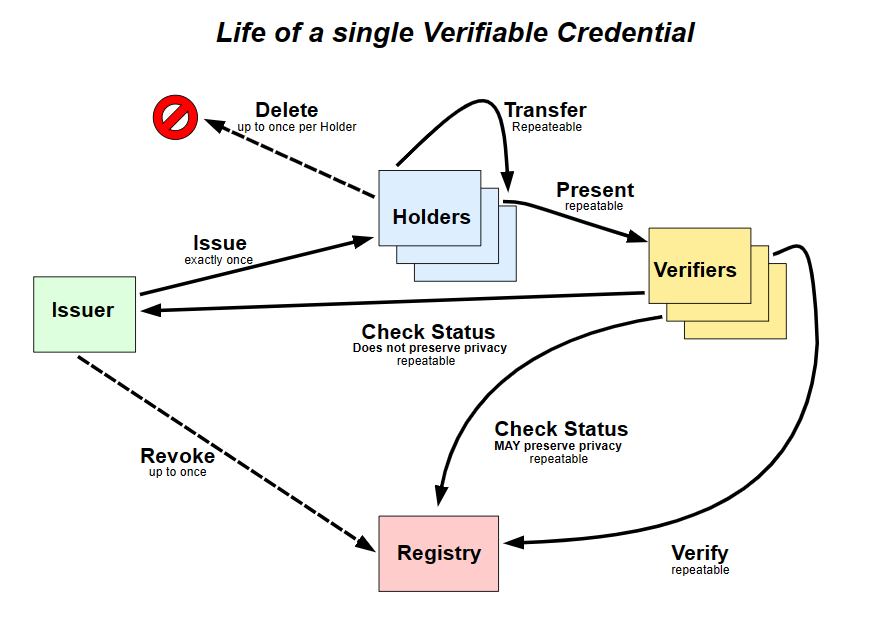
\includegraphics[scale = 1]{./res/images/Immaginew3c.png}
\end{center}

\subsection{Esempi}
Un esempio di grande dataset:
\begin{itemize}
    \item un tipico caso di un grande dataset collegato è DBPedia, che, fondamentalmente, rende disponibile il contenuto di Wikipedia in formato RDF. L'importanza di DBPedia non è solo quella di includere i dati di Wikipedia, ma anche quella di incorporare collegamenti ad altri dataset sul Web, ad esempio a Geonames. Fornendo questi collegamenti aggiuntivi (sotto forma di triple RDF), le applicazioni possono sfruttare le conoscenze extra (e possibilmente più precise) provenienti da altri dataset durante lo sviluppo di un'applicazione; grazie all'integrazione di informazioni provenienti da diversi dataset, l'applicazione può offrire un'esperienza utente molto migliore.
\end{itemize}

Di seguito sono elencati alcuni esempi di come il W3C Data Model potrebbe essere applicato a un ipotetico portafoglio digitale che raccoglie le credenziali d'accesso degli utenti, come ad esempio il Sistema Pubblico di Identità Digitale (SPID):
\begin{itemize}
    \item \textbf{Rappresentazione delle credenziali}: utilizzando il W3C Data Model, il portafoglio digitale potrebbe rappresentare le credenziali d'accesso come oggetti RDF. Ad esempio, un oggetto RDF potrebbe rappresentare una specifica credenziale SPID con proprietà come "codice fiscale", "username", "password" e "scadenza";
    \item \textbf{Ontologia delle credenziali}: potrebbe essere utilizzata un'ontologia basata sul W3C Data Model per definire i concetti e le relazioni all'interno del portafoglio digitale. Questa ontologia potrebbe includere classi come "Credenziale", "Provider di Identità" e proprietà come "tipo di autenticazione" e "livello di affidabilità";
    \item \textbf{Annotazione semantica dei dati}: attraverso l'uso delle triple RDF, il portafoglio digitale potrebbe essere arricchito con metadati semantici per fornire ulteriori informazioni sulle credenziali. Ad esempio, potrebbero essere aggiunti metadati come "data di registrazione" o "ultima modifica" per tenere traccia delle attività relative alle credenziali;
    \item \textbf{Query e interrogazione}: utilizzando il linguaggio di interrogazione SPARQL, sarebbe possibile eseguire interrogazioni sulle credenziali nel portafoglio digitale. Ad esempio, si potrebbero recuperare tutte le credenziali associate a un determinato codice fiscale o controllare la validità di una specifica credenziale;
    \item \textbf{Esportazione e importazione dei dati}: il W3C Data Model consentirebbe l'esportazione e l'importazione dei dati del portafoglio digitale delle credenziali in diversi formati standard, come RDF/XML o Turtle. Ciò permetterebbe lo scambio dei dati con altri sistemi o applicazioni che utilizzano lo stesso modello di dati;
    \item \textbf{Privacy e sicurezza}: il W3C Data Model supporta anche questioni di privacy e sicurezza. Attraverso l'utilizzo di politiche di accesso controllato, crittografia e tecnologie di autenticazione, le credenziali sensibili nel portafoglio digitale potrebbero essere protette e accessibili solo agli utenti autorizzati;
    \item \textbf{Integrazione con servizi di autenticazione}: utilizzando il W3C Data Model, il portafoglio digitale potrebbe integrarsi con servizi di autenticazione basati su SPID o altri protocolli. Ad esempio, il portafoglio potrebbe fornire un'interfaccia per consentire all'utente di utilizzare le proprie credenziali SPID per l'autenticazione su piattaforme o applicazioni compatibili.
\end{itemize}

\subsection{Esempi di codice}
Per illustrare il ciclo di vita di una Verifiable Credential, useremo l'esempio del riscatto di uno sconto per ex studenti da parte di un'università. Nell'esempio seguente, Pat riceve una credenziale verificabile da ex studente da un'università e Pat memorizza la credenziale verificabile in un portafoglio digitale.\\

Un semplice esempio di una credenziale verificabile:
\begin{verbatim}
    {
  // set the context, which establishes the special terms we will be using
  // such as 'issuer' and 'alumniOf'.
  "@context": [
    "https://www.w3.org/2018/credentials/v1",
    "https://www.w3.org/2018/credentials/examples/v1"
  ],
  // specify the identifier for the credential
  "id": "http://example.edu/credentials/1872",
  // the credential types, which declare what data to expect in the credential
  "type": ["VerifiableCredential", "AlumniCredential"],
  // the entity that issued the credential
  "issuer": "https://example.edu/issuers/565049",
  // when the credential was issued
  "issuanceDate": "2010-01-01T19:23:24Z",
  // claims about the subjects of the credential
  "credentialSubject": {
    // identifier for the only subject of the credential
    "id": "did:example:ebfeb1f712ebc6f1c276e12ec21",
    // assertion about the only subject of the credential
    "alumniOf": {
      "id": "did:example:c276e12ec21ebfeb1f712ebc6f1",
      "name": [{
        "value": "Example University",
        "lang": "en"
      }, {
        "value": "Exemple d'Université",
        "lang": "fr"
      }]
    }
  },
  // digital proof that makes the credential tamper-evident
  // see the NOTE at end of this section for more detail
  "proof": {
    // the cryptographic signature suite that was used to generate the signature
    "type": "RsaSignature2018",
    // the date the signature was created
    "created": "2017-06-18T21:19:10Z",
    // purpose of this proof
    "proofPurpose": "assertionMethod",
    // the identifier of the public key that can verify the signature
    "verificationMethod": "https://example.edu/issuers/565049#key-1",
    // the digital signature value
    "jws": "eyJhbGciOiJSUzI1NiIsImI2NCI6ZmFsc2UsImNyaXQiOlsiYjY0Il19..TCYt5X
      sITJX1CxPCT8yAV-TVkIEq_PbChOMqsLfRoPsnsgw5WEuts01mq-pQy7UJiN5mgRxD-WUc
      X16dUEMGlv50aqzpqh4Qktb3rk-BuQy72IFLOqV0G_zS245-kronKb78cPN25DGlcTwLtj
      PAYuNzVBAh4vGHSrQyHUdBBPM"
  }
}
\end{verbatim}
Successivamente, Pat cerca di riscattare lo sconto per ex studenti. Il verificatore, un sistema di vendita di biglietti, afferma che ogni ex studente dell'"Example University" riceve uno sconto sui biglietti stagionali per gli eventi sportivi. Utilizzando un dispositivo mobile, Pat avvia il processo di acquisto di un abbonamento stagionale. Durante una fase di questo processo, viene richiesta una credenziale verificabile da ex studente, e questa richiesta viene inviata al portafoglio digitale di Pat. Il portafoglio digitale chiede a Pat se desidera fornire una credenziale verificabile precedentemente emessa. Pat seleziona la credenziale verificabile da ex studente, che viene quindi composta in una presentazione verificabile. La presentazione verificabile viene inviata al verificatore e viene verificata.\\

Un semplice esempio di una presentazione verificabile:
\begin{verbatim}
    {
  "@context": [
    "https://www.w3.org/2018/credentials/v1",
    "https://www.w3.org/2018/credentials/examples/v1"
  ],
  "type": "VerifiablePresentation",
  // the verifiable credential issued in the previous example
  "verifiableCredential": [{
    "@context": [
      "https://www.w3.org/2018/credentials/v1",
      "https://www.w3.org/2018/credentials/examples/v1"
    ],
    "id": "http://example.edu/credentials/1872",
    "type": ["VerifiableCredential", "AlumniCredential"],
    "issuer": "https://example.edu/issuers/565049",
    "issuanceDate": "2010-01-01T19:23:24Z",
    "credentialSubject": {
      "id": "did:example:ebfeb1f712ebc6f1c276e12ec21",
      "alumniOf": {
        "id": "did:example:c276e12ec21ebfeb1f712ebc6f1",
        "name": [{
          "value": "Example University",
          "lang": "en"
        }, {
          "value": "Exemple d'Université",
          "lang": "fr"
        }]
      }
    },
    "proof": {
      "type": "RsaSignature2018",
      "created": "2017-06-18T21:19:10Z",
      "proofPurpose": "assertionMethod",
      "verificationMethod": "https://example.edu/issuers/565049#key-1",
      "jws": "eyJhbGciOiJSUzI1NiIsImI2NCI6ZmFsc2UsImNyaXQiOlsiYjY0Il19..TCYt5X
        sITJX1CxPCT8yAV-TVkIEq_PbChOMqsLfRoPsnsgw5WEuts01mq-pQy7UJiN5mgRxD-WUc
        X16dUEMGlv50aqzpqh4Qktb3rk-BuQy72IFLOqV0G_zS245-kronKb78cPN25DGlcTwLtj
        PAYuNzVBAh4vGHSrQyHUdBBPM"
    }
  }],
  // digital signature by Pat on the presentation
  // protects against replay attacks
  "proof": {
    "type": "RsaSignature2018",
    "created": "2018-09-14T21:19:10Z",
    "proofPurpose": "authentication",
    "verificationMethod": "did:example:ebfeb1f712ebc6f1c276e12ec21#keys-1",
    // 'challenge' and 'domain' protect against replay attacks
    "challenge": "1f44d55f-f161-4938-a659-f8026467f126",
    "domain": "4jt78h47fh47",
    "jws": "eyJhbGciOiJSUzI1NiIsImI2NCI6ZmFsc2UsImNyaXQiOlsiYjY0Il19..kTCYt5
      XsITJX1CxPCT8yAV-TVIw5WEuts01mq-pQy7UJiN5mgREEMGlv50aqzpqh4Qq_PbChOMqs
      LfRoPsnsgxD-WUcX16dUOqV0G_zS245-kronKb78cPktb3rk-BuQy72IFLN25DYuNzVBAh
      4vGHSrQyHUGlcTwLtjPAnKb78"
  }
}
\end{verbatim}

Esempio preso dal sito ufficiale del W3C:\\
\url{https://www.w3.org/TR/vc-data-model/#proof-formats}\\